\chapter{Progetto Interconnect}

Il progetto Interconnect ha l'obiettivo di introdurre concetti per l'interoperabilità e l'integrazione dei dati da diverse fonti, in modo che gli utenti possano fornire i propri servizi e accedere a informazioni pertinenti e correlate in modo più efficiente.


\section{Ontologie Interconnect}
Interconnect non è una singola ontologia, è una famiglia di ontologie che si basano sull'uso di ontologie già esistenti (in particolare SAREF e relative estensioni per l'energia).
Nella figura \ref{fig:panoramicaInterconnect} viene raffigurata una panoramica sulle ontologie create all'interno del progetto, mostrando le altre ontologie utilizzate ed estese. In particolare si può notare la famiglia SAREF di ETSI (SAREF e relative estensioni già trattate nel capitolo \ref{cap:panoramicaSaref}).
\begin{figure}[H]
    \centering
    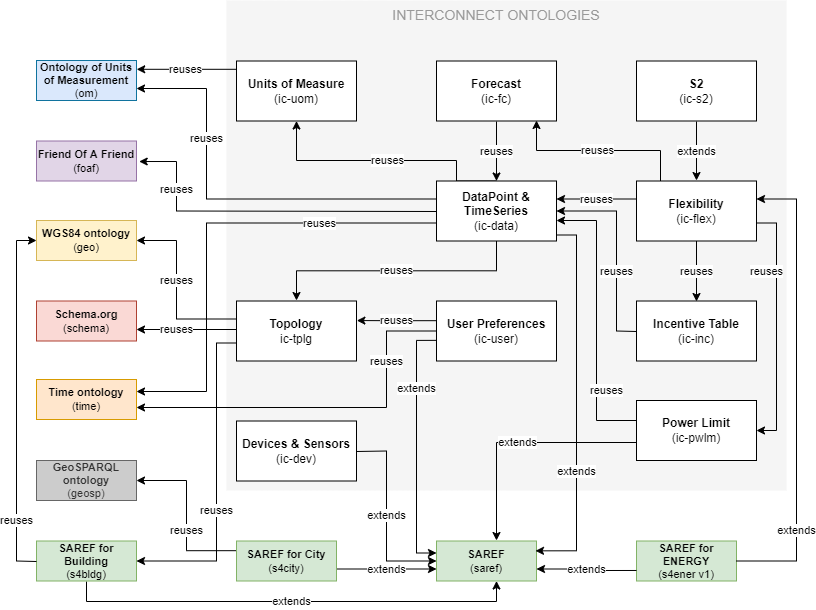
\includegraphics[width=\textwidth]{figures/panoramicaInterconnect.png}
    \caption{Panoramica delle ontologie InterConnect in relazione a SAREF e ad altre ontologie esistenti.}
    \label{fig:panoramicaInterconnect}
\end{figure}

\subsection{Ontologie create nel progetto Interconnect}
Nel progetto Interconnect sono state sviluppate nove ontologie. Vengono presentate nella tabella \ref{tab:ontologieCreate}
\begin{table}[H]
    \centering
    \begin{tabularx}{\textwidth}{|X|X|X|}
        \hline
        Prefisso & Namespace                                                         & Concetti                                                                                            \\
        \hline
        ic-data  & \href{http://ontology.tno.nl/interconnect/datapoint\#}{link}      & Datapoint, TimeSeries, Message, Utility Purpose                                                     \\
        ic-dev   & \href{http://ontology.tno.nl/interconnect/device\#}{link}         & Device, State, Function                                                                             \\
        ic-flex  & \href{http://ontology.tno.nl/interconnect/flexibility\#}{link}    & Flex Offer, Flexibility Source, Control Type, Power Envelope                                        \\
        ic-fc    & \href{http://ontology.tno.nl/interconnect/forecast\#}{link}       & Forecast, Point Forecast, Stochastic Forecast (Gaussian, Quantile, Trajectory), Gaussian Data Point \\
        ic-inc   & \href{http://ontology.tno.nl/interconnect/incentivetable\#}{link} & Incentive Table, Incentive Tiers, Scope and Type                                                    \\
        ic-pwlm  & \href{http://ontology.tno.nl/interconnect/powerlimit\#}{link}     & Power Limit (Nominal, Contractual and Failsafe)                                                     \\
        ic-tplg  & \href{http://ontology.tno.nl/interconnect/topology\#}{link}       & Topological Location, Grid Segment, Market Segment, Regulation Zone, Electrical Phases              \\
        ic-uom   & \href{http://ontology.tno.nl/interconnect/units\#}{link}          & Additional Units of Measure (not considered yet in SAREF)                                           \\
        ic-user  & \href{http://ontology.tno.nl/interconnect/user\#}{link}           & User, User Profile, Preference, Priority, Interest, Activity, Time, Location                        \\
        \hline
    \end{tabularx}
    \caption{Ontologie create all'interno del progetto Interconnect}
    \label{tab:ontologieCreate}
\end{table}

\subsection{Ontologie utilizzate}
L'utilizzo di altre ontologie è uno dei pilastri del web semantico. Nella tabella \ref{tab:ontologieUtilizzate} vengono elencate tutte le ontologie utilizzate nel progetto Interconnect, con relativo dettaglio sui concetti di tali librerie.
\begin{table}[H]
    \centering
    \begin{tabularx}{\textwidth}{|X|X|X|}
        \hline
        Prefisso & Namespace                                                               & Concetti                                                                            \\
        \hline
        foaf     & \href{http://xmlns.com/foaf/0.1/}{link}                                 & Agent                                                                               \\
        geo      & \href{http://www.w3.org/2003/01/geo/wgs84_pos}{link}                    & Spatial Thing, geo coordinates                                                      \\
        geosp    & \href{http://www.opengis.net/ont/geosparql}{link}                       & Geographical Feature                                                                \\
        schema   & \href{https://schema.org/}{link}                                        & Address, Countries, Postal Codes                                                    \\
        om       & \href{http://www.ontology-of-units-of-measure.org/resource/om-2/}{link} & Quantity, Unit, Measure                                                             \\
        saref    & \href{https://saref.etsi.org/core/}{link}                               & Device, Function, Command, State, Measurement, Unit of Measure, Feature of Interest \\
        s4bldg   & \href{https://saref.etsi.org/saref4bldg/}{link}                         & Building, Building Space, Building Object                                           \\
        s4city   & \href{https://saref.etsi.org/saref4ener/}{link}                         & Power Profile, Alternatives, Power Sequence, Slot                                   \\
        s4ener   & \href{https://saref.etsi.org/saref4city/}{link}                         & Facility, Administrative Area, City Object                                          \\
        time     & \href{http://www.w3.org/2006/time}{link}                                & Instant, Interval, Duration                                                         \\
        \hline
    \end{tabularx}
    \caption{Ontologie utilizzate all'interno del progetto Interconnect}
    \label{tab:ontologieUtilizzate}
\end{table}

\section{InterConnect Interoperability Framework}
La parte interessante di questo progetto è l'Interoperability Framework che viene fornito.
Questo Interoperability Framework è capace di colmare le lacune di interoperabilità all'interno e tra i domini dell'energia e dell'IoT.

\begin{figure}[H]
    \centering
    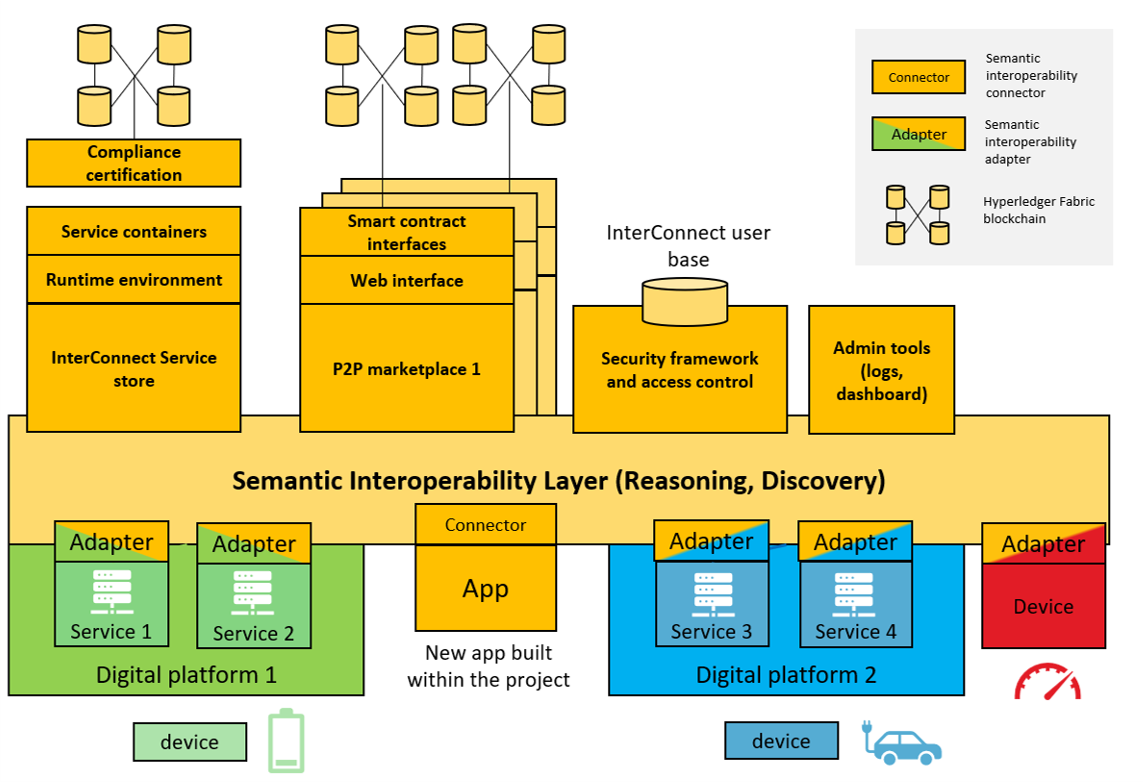
\includegraphics[width=\textwidth]{figures/architetturaFrameworkInterconnect.png}
    \caption{Architettura di alto livello dell'InterConnect Interoperability Framework.}
    \label{fig:architetturaFrameworkInterconnect}
\end{figure}

Di seguito vengono elencati i tre componenti principali del Framework:
\begin{itemize}
    \item InterConnect Service Store;
    \item Semantic Interoperability Layer;
    \item P2P MarketPlace.
\end{itemize}

\paragraph{InterConnect Service Store}

Il Service Store non è altro che un'applicazione web dove è necessario registrarsi per poter utilizzare o fornire servizi in maniera interoperabile, sia provenienti da settori energetici che non energetici. È possibile accedervi dal seguente \href{https://store.interconnectproject.eu/ServiceStore}{link}.

L'obiettivo principale è quello di favorire lo sviluppo dell'ecosistema InterConnect, in cui fornitori e utilizzatori di servizi possano collaborare in modo più efficace. Questo sarà possibile grazie alla possibilità di registrare nuovi servizi interoperabili e di consultare quelli già esistenti, al fine di individuare quelli più adatti alle proprie esigenze e di ottenere tutte le informazioni necessarie per accedere e utilizzare correttamente i servizi selezionati. In questo modo, si creerà un punto di riferimento unico per tutti gli utenti dell'ecosistema InterConnect, con benefici in termini di semplificazione dell'accesso alle informazioni e miglioramento della qualità dei servizi offerti.


\paragraph{Semantic Interoperability Layer (SIL)}
Il Semantic Interoperability Layer è il componente principale del framework. È responsabile dello scambio di conoscenza tra tutti i componenti e servizi interoperabili.
Il SIL è composto da più moduli, elencati di seguito:
\begin{itemize}
    \item knowdlege engine: responsabile dello scambio di dati tra I servizi;
    \item Generic adapter: il middleware che deve essere collegato a ogni servizio per rendere il servizio interoperabile;
    \item Ontologie: vanno usate ontologie già esistenti (ad esempio saref) per definire uno standard per il dominio;
    \item Discovery: per mettere a disposizione i propri servizi e per vedere i servizi disponibili a essere utilizzati;
\end{itemize}


\paragraph{P2P MarketPlace}
